% Original vector reconstruction of source Fig.80.3, PDF325 / printed313.
% All three panels have counterclockwise external order (1,2,3,4).
% Internal edges carry k1+k2 and k1+k4 respectively; arrows only carry color.
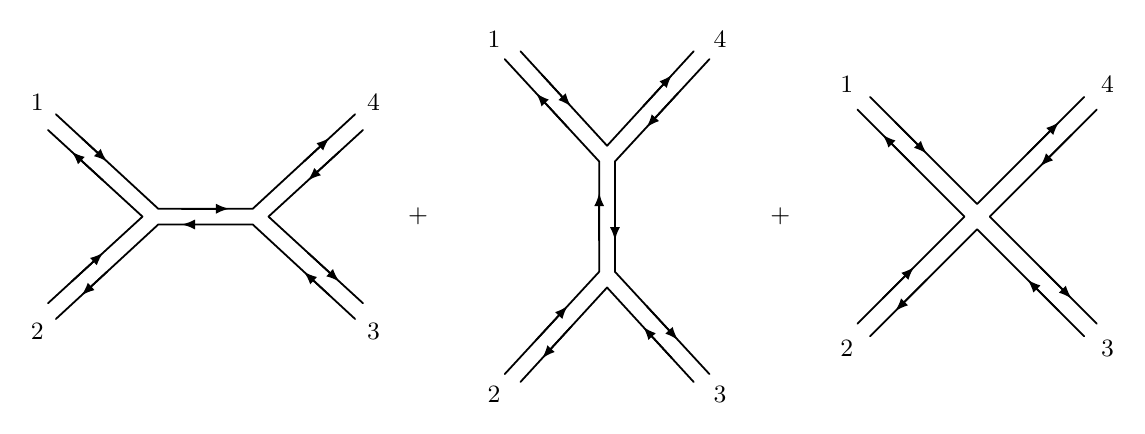
\begin{tikzpicture}[x=1mm,y=1mm,line width=.65pt,>=latex,
 line cap=round,line join=round,font=\fontsize{9.5}{11}\selectfont]
\begin{scope}[shift={(24,0)}]
  \draw (-19,13)--(-6,1)--(6,1)--(19,13);
  \draw (-19,-13)--(-6,-1)--(6,-1)--(19,-13);
  \draw (-20,11)--(-8,0)--(-20,-11);
  \draw (20,11)--(8,0)--(20,-11);
  \draw[->] (-15.75,10)--(-12.5,7);
  \draw[->] (-13,4.58333)--(-17,8.25);
  \draw[->] (-17,-8.25)--(-13,-4.58333);
  \draw[->] (-12.5,-7)--(-15.75,-10);
  \draw[->] (12.5,7)--(15.75,10);
  \draw[->] (17,8.25)--(13,4.58333);
  \draw[->] (13,-4.58333)--(17,-8.25);
  \draw[->] (15.75,-10)--(12.5,-7);
  \draw[->] (-3,1)--(3,1);
  \draw[->] (3,-1)--(-3,-1);
  \node[above left,inner sep=1.2pt] at (-20,13) {$1$};
  \node[below left,inner sep=1.2pt] at (-20,-13) {$2$};
  \node[below right,inner sep=1.2pt] at (20,-13) {$3$};
  \node[above right,inner sep=1.2pt] at (20,13) {$4$};
\end{scope}
\node at (51,0) {$+$};
\begin{scope}[shift={(75,0)}]
  \draw (-13,20)--(-1,7)--(-1,-7)--(-13,-20);
  \draw (13,20)--(1,7)--(1,-7)--(13,-20);
  \draw (-11,21)--(0,9)--(11,21);
  \draw (-11,-21)--(0,-9)--(11,-21);
  \draw[->] (-5,11.33333)--(-9,15.66667);
  \draw[->] (-8.25,18)--(-4.58333,14);
  \draw[->] (4.58333,14)--(8.25,18);
  \draw[->] (9,15.66667)--(5,11.33333);
  \draw[->] (-9,-15.66667)--(-5,-11.33333);
  \draw[->] (-4.58333,-14)--(-8.25,-18);
  \draw[->] (5,-11.33333)--(9,-15.66667);
  \draw[->] (8.25,-18)--(4.58333,-14);
  \draw[->] (-1,-3)--(-1,3);
  \draw[->] (1,3)--(1,-3);
  \node[above left,inner sep=1.2pt] at (-13,21) {$1$};
  \node[below left,inner sep=1.2pt] at (-13,-21) {$2$};
  \node[below right,inner sep=1.2pt] at (13,-21) {$3$};
  \node[above right,inner sep=1.2pt] at (13,21) {$4$};
\end{scope}
\node at (97,0) {$+$};
\begin{scope}[shift={(122,0)},scale=.8]
  \draw (-17,19)--(0,2)--(17,19);
  \draw (-19,17)--(-2,0)--(-19,-17);
  \draw (-17,-19)--(0,-2)--(17,-19);
  \draw (19,17)--(2,0)--(19,-17);
  \draw[->] (-13,15)--(-8,10);
  \draw[->] (-10,8)--(-15,13);
  \draw[->] (8,10)--(13,15);
  \draw[->] (15,13)--(10,8);
  \draw[->] (-15,-13)--(-10,-8);
  \draw[->] (-8,-10)--(-13,-15);
  \draw[->] (10,-8)--(15,-13);
  \draw[->] (13,-15)--(8,-10);
  \node[above left,inner sep=1.2pt] at (-19,19) {$1$};
  \node[below left,inner sep=1.2pt] at (-19,-19) {$2$};
  \node[below right,inner sep=1.2pt] at (19,-19) {$3$};
  \node[above right,inner sep=1.2pt] at (19,19) {$4$};
\end{scope}
\end{tikzpicture}
